%\PassOptionsToPackage{draft}{graphicx}
%\documentclass[10pt]{beamer} % aspect ratio 4:3, 128 mm by 96 mm
\documentclass[10pt,aspectratio=169]{beamer} % aspect ratio 16:9
%\graphicspath{{../../figures/}}
\graphicspath{{figs/}}
%\includeonlyframes{frame1,frame2,frame3}

%%%%%%%%%%%%%%%%%%%%%%%%%%%%%%%%%%%%%%%%%%%%%%%%%%
% Packages
%%%%%%%%%%%%%%%%%%%%%%%%%%%%%%%%%%%%%%%%%%%%%%%%%%
\usepackage{appendixnumberbeamer}
\usepackage{booktabs}
\usepackage{csvsimple} % for csv read
\usepackage[scale=2]{ccicons}
\usepackage{pgfplots}
\usepackage{xspace}
\usepackage{amsmath}
\usepackage{totcount}
\usepackage{tikz}
\usepackage{bm}
\usepackage{float}
\usepackage{eso-pic} 
\usepackage{wrapfig}
\usepackage{animate,media9,movie15}
\usepackage{subfig}

\usepackage{multimedia}
%\usepackage{FiraSans}

%\usepackage{comment}
%\usetikzlibrary{external} % speedup compilation
%\tikzexternalize % activate!
%\usetikzlibrary{shapes,arrows}  

%\usepackage{bibentry}
%\nobibliography*
\usepackage{ifthen}
\newcounter{angle}
\setcounter{angle}{0}
%\usepackage{bibentry}
%\nobibliography*
\usepackage{caption}%

\captionsetup[figure]{labelformat=empty}%
\graphicspath{{figures/}}
\usefonttheme{structurebold}
%%%%%%%%%%%%%%%%%%%%%%%%%%%%%%%%%%%%%%%%%%%%%%%%%%
% Metropolis theme custom modification file
%%%%%%%%%%%%%%%%%%%%%%%%%%%%%%%%%%%%%%%%%%%%%%%%%%
% Metropolis theme custom modification file
%%%%%%%%%%%%%%%%%%%%%%%%%%%%%%%%%%%%%%%%%%%%%%%%%%
% Metropolis theme custom colors
%%%%%%%%%%%%%%%%%%%%%%%%%%%%%%%%%%%%%%%%%%%%%%%%%%
\usetheme[progressbar=foot]{metropolis}
\useoutertheme{metropolis}
\useinnertheme{metropolis}
\usefonttheme{metropolis}
\setbeamercolor{background canvas}{bg=white}

%\usecolortheme{spruce}

\definecolor{myblue}{rgb}{0.19,0.55,0.91}
\definecolor{mediumblue}{rgb}{0,0,205}
\definecolor{darkblue}{rgb}{0,0,139}
\definecolor{Dodgerblue}{HTML}{1E90FF}
\definecolor{Navy}{HTML}{000080} % {rgb}{0,0,128}
\definecolor{Aliceblue}{HTML}{F0F8FF}
\definecolor{Lightskyblue}{HTML}{87CEFA}
\definecolor{logoblue}{RGB}{1,67,140}
\definecolor{Purple}{HTML}{911146}
\definecolor{Orange}{HTML}{CF4A30}

\setbeamercolor{progress bar}{bg=Lightskyblue}
\setbeamercolor{progress bar}{ fg=logoblue} 
\setbeamercolor{frametitle}{bg=logoblue}
\setbeamercolor{title separator}{fg=logoblue}
\setbeamercolor{block title}{bg=Lightskyblue!30,fg=black}
\setbeamercolor{block body}{bg=Lightskyblue!15,fg=black}
\setbeamercolor{alerted text}{fg=Purple}
% notes colors
\setbeamercolor{note page}{bg=white}
\setbeamercolor{note title}{bg=Lightskyblue}
%%%%%%%%%%%%%%%%%%%%%%%%%%%%%%%%%%%%%%%%%%%%%%%%%%
%  Theme modifications
%%%%%%%%%%%%%%%%%%%%%%%%%%%%%%%%%%%%%%%%%%%%%%%%%%
% modify progress bar linewidth
\makeatletter
\setlength{\metropolis@progressinheadfoot@linewidth}{2pt} 
\setlength{\metropolis@titleseparator@linewidth}{1pt}
\setlength{\metropolis@progressonsectionpage@linewidth}{1pt}

\setbeamertemplate{progress bar in section page}{
	\setlength{\metropolis@progressonsectionpage}{%
		\textwidth * \ratio{\thesection pt}{\totvalue{totalsection} pt}%
	}%
	\begin{tikzpicture}
		\fill[bg] (0,0) rectangle (\textwidth, 
		\metropolis@progressonsectionpage@linewidth);
		\fill[fg] (0,0) rectangle (\metropolis@progressonsectionpage, 
		\metropolis@progressonsectionpage@linewidth);
	\end{tikzpicture}%
}
\makeatother
\newcounter{totalsection}
\regtotcounter{totalsection}

\AtBeginDocument{%
	\pretocmd{\section}{\refstepcounter{totalsection}}{\typeout{Yes, prepending 
	was successful}}{\typeout{No, prepending was not successful}}%
}%
%%%%%%%%%%%%%%%%%%%%%%%%%%%%%%%%%%%%%%%%%%%%%%%%%%
%  Bibliography mods
%%%%%%%%%%%%%%%%%%%%%%%%%%%%%%%%%%%%%%%%%%%%%%%%%%
\setbeamertemplate{bibliography item}{\insertbiblabel} %% Remove book symbol 
%%from references and add number in square brackets
% kill the abominable icon (without number)
%\setbeamertemplate{bibliography item}{}
%\makeatletter
%\renewcommand\@biblabel[1]{#1.} % number only
%\makeatother
% remove line breaks in bibliography
\setbeamertemplate{bibliography entry title}{}
\setbeamertemplate{bibliography entry location}{}
%%%%%%%%%%%%%%%%%%%%%%%%%%%%%%%%%%%%%%%%%%%%%%%%%%
%  Bibliography custom commands
%%%%%%%%%%%%%%%%%%%%%%%%%%%%%%%%%%%%%%%%%%%%%%%%%%
\newcommand{\bibliotitlestyle}[1]{\textbf{#1}\par}

\newif\ifinbiblio
\newcounter{bibkey}
\newenvironment{biblio}[2][long]{%
	%\setbeamertemplate{bibliography item}{\insertbiblabel}
	\setbeamertemplate{bibliography item}{}% without numbers
	\setbeamerfont{bibliography item}{size=\footnotesize}
	\setbeamerfont{bibliography entry author}{size=\footnotesize}
	\setbeamerfont{bibliography entry title}{size=\footnotesize}
	\setbeamerfont{bibliography entry location}{size=\footnotesize}
	\setbeamerfont{bibliography entry note}{size=\footnotesize}
	\ifx!#2!\else%
	\bibliotitlestyle{#2}%
	\fi%
	\begin{thebibliography}{}%
		\inbibliotrue%
		\setbeamertemplate{bibliography entry title}[#1]%
	}{%
		\inbibliofalse%
		\setbeamertemplate{bibliography item}{}%
	\end{thebibliography}%
}

\newcommand{\biblioref}[5][short]{
	\setbeamertemplate{bibliography entry title}[#1]
	\stepcounter{bibkey}%
	\ifinbiblio%
	\bibitem{\thebibkey}%
	#2
	\newblock #4
	\ifx!#5!\else\newblock {\em #5}, #3 \fi%
	\else%
	\begin{biblio}{}
		\bibitem{\thebibkey}
		#2
		\newblock #4
		\ifx!#5!\else\newblock {\em #5}, #3\fi
	\end{biblio}
	\fi
}
%
%\newbibmacro*{hypercite}{%
%	\renewcommand{\@makefntext}[1]{\noindent\normalfont##1}%
%	\footnotetext{%
%		\blxmkbibnote{foot}{%
%			\printtext[labelnumberwidth]{%
%				\printfield{prefixnumber}%
%				\printfield{labelnumber}}%
%			\addspace
%			\fullcite{\thefield{entrykey}}}}}
%
%\DeclareCiteCommand{\hypercite}%
%{\usebibmacro{cite:init}}
%{\usebibmacro{hypercite}}
%{}
%{\usebibmacro{cite:dump}}
%
%% Redefine the \footfullcite command to use the reference number
%\renewcommand{\footfullcite}[1]{\cite{#1}\hypercite{#1}}
%\usefonttheme[onlymath]{Serif}  % It should be uncommented if Fira fonts in 
%%math does not work

%%%%%%%%%%%%%%%%%%%%%%%%%%%%%%%%%%%%%%%%%%%%%%%%%%
% Custom commands
%%%%%%%%%%%%%%%%%%%%%%%%%%%%%%%%%%%%%%%%%%%%%%%%%%
% matrix command 
\newcommand{\matr}[1]{\mathbf{#1}} % bold upright (Elsevier, Springer)
%\newcommand{\matr}[1]{#1}          % pure math version
%\newcommand{\matr}[1]{\bm{#1}}     % ISO complying version
% vector command 
\newcommand{\vect}[1]{\mathbf{#1}} % bold upright (Elsevier, Springer)
% bold symbol
\newcommand{\bs}[1]{\boldsymbol{#1}}
% derivative upright command
\DeclareRobustCommand*{\drv}{\mathop{}\!\mathrm{d}}
\newcommand{\ud}{\mathrm{d}}
% 
\newcommand{\themename}{\textbf{\textsc{metropolis}}\xspace}

%%%%%%%%%%%%%%%%%%%%%%%%%%%%%%%%%%%%%%%%%%%%%%%%%%
%  Title page options
%%%%%%%%%%%%%%%%%%%%%%%%%%%%%%%%%%%%%%%%%%%%%%%%%%
% \date{\today}
\date{}
%%%%%%%%%%%%%%%%%%%%%%%%%%%%%%%%%%%%%%%%%%%%%%%%%%
% option 1
%%%%%%%%%%%%%%%%%%%%%%%%%%%%%%%%%%%%%%%%%%%%%%%%%%%
\title{Deep learning for damage identification in CFRP materials}
\subtitle{Feasibility studies of artificial intelligence driven diagnostics}
\author{\textbf{Abdalraheem Ijjeh\\Supervisor: Prof. Paweł Kudela}}
% logo align to Institute 
\institute{Institute of Fluid Flow Machinery \\ 
	Polish Academy of Sciences \\ 
	\vspace{-1.5cm}
	\flushright 
	\includegraphics[width=6cm]{imp_logo.png}}
%%%%%%%%%%%%%%%%%%%%%%%%%%%%%%%%%%%%%%%%%%%%%%%%%%
% option 2 - authors in one line
%%%%%%%%%%%%%%%%%%%%%%%%%%%%%%%%%%%%%%%%%%%%%%%%%%
%	\title{My fancy title}
%	\subtitle{Lamb-opt}
%	\author{\textbf{Paweł Kudela}\textsuperscript{2}, Maciej 
%	Radzieński\textsuperscript{2}, Wiesław Ostachowicz\textsuperscript{2}, 
%	Zhibo Yang\textsuperscript{1} }
%	 logo align to Institute 
%	\institute{\textsuperscript{1}Xi'an Jiaotong University \\ 
%	\textsuperscript{2}Institute of Fluid Flow Machinery\\ \hspace*{1pt} Polish 
%	Academy of Sciences \\ \vspace{-1.5cm}\flushright 
%	
%\includegraphics[width=4cm]{//odroid-sensors/sensors/MISD_shared/logo/logo_eng_40mm.eps}}
%%%%%%%%%%%%%%%%%%%%%%%%%%%%%%%%%%%%%%%%%%%%%%%%%%%
% option 3 - multilogo vertical
%%%%%%%%%%%%%%%%%%%%%%%%%%%%%%%%%%%%%%%%%%%%%%%%%%
%%\title{My fancy title}
%%\subtitle{Lamb-opt}
%%	\author{\textbf{Paweł Kudela}\inst{1}, Maciej Radzieński\inst{1}, Wiesław Ostachowicz\inst{1}, Zhibo Yang\inst{2} }
%%	 logo under Institute 
%%	\institute%
%%	{ 
%%		\inst{1}%
%%		Institute of Fluid Flow Machinery\\ \hspace*{1pt} Polish Academy of Sciences \\ \includegraphics[height=0.85cm]{//odroid-sensors/sensors/MISD_shared/logo/logo_eng_40mm.eps} \\
%%		\and
%%		\inst{2}%
%%	    Xi'an Jiaotong University \\ \includegraphics[height=0.85cm]{//odroid-sensors/sensors/MISD_shared/logo/logo_box.eps}
%%    }
% end od option 3
%%%%%%%%%%%%%%%%%%%%%%%%%%%%%%%%%%%%%%%%%%%%%%%%%%
%% option 4 - 3 Institutes and logos horizontal centered
%%%%%%%%%%%%%%%%%%%%%%%%%%%%%%%%%%%%%%%%%%%%%%%%%%
%\title{My fancy title}
%\subtitle{Lamb-opt }
%\author{\textbf{Paweł Kudela}\textsuperscript{1}, Maciej Radzieński\textsuperscript{1}, Marco Miniaci\textsuperscript{2}, Zhibo Yang\textsuperscript{3} }
%
%\institute{ 
%\begin{columns}[T,onlytextwidth]
%	\column{0.39\textwidth}
%	\begin{center}
%		\textsuperscript{1}Institute of Fluid Flow Machinery\\ \hspace*{3pt}Polish Academy of Sciences
%	\end{center}
%	\column{0.3\textwidth}
%	\begin{center}
%		\textsuperscript{2}Zurich University
%	\end{center}
%	\column{0.3\textwidth}
%	\begin{center}
%		\textsuperscript{3}Xi'an Jiaotong University
%	\end{center}
%\end{columns}
%\vspace{6pt}
%% logos 
%\begin{columns}[b,onlytextwidth]
%	\column{0.39\textwidth}
%		\centering 
%		\includegraphics[scale=0.9,height=0.85cm,keepaspectratio]{//odroid-sensors/sensors/MISD_shared/logo/logo_eng_40mm.eps}
%	\column{0.3\textwidth}
%		\centering 
%		\includegraphics[scale=0.9,height=0.85cm,keepaspectratio]{//odroid-sensors/sensors/MISD_shared/logo/logo_box.eps}
%	\column{0.3\textwidth}
%		\centering 
%		\includegraphics[scale=0.9,height=0.85cm,keepaspectratio]{//odroid-sensors/sensors/MISD_shared/logo/logo_box2.eps}
%\end{columns}
%}
%\makeatletter
%\setbeamertemplate{title page}{
%	\begin{minipage}[b][\paperheight]{\textwidth}
%		\centering  % <-- Center here
%		\ifx\inserttitlegraphic\@empty\else\usebeamertemplate*{title graphic}\fi
%		\vfill%
%		\ifx\inserttitle\@empty\else\usebeamertemplate*{title}\fi
%		\ifx\insertsubtitle\@empty\else\usebeamertemplate*{subtitle}\fi
%		\usebeamertemplate*{title separator}
%		\ifx\beamer@shortauthor\@empty\else\usebeamertemplate*{author}\fi
%		\ifx\insertdate\@empty\else\usebeamertemplate*{date}\fi
%		\ifx\insertinstitute\@empty\else\usebeamertemplate*{institute}\fi
%		\vfill
%		\vspace*{1mm}
%	\end{minipage}
%}
%
%\setbeamertemplate{title}{
%	%  \raggedright%  % <-- Comment here
%	\linespread{1.0}%
%	\inserttitle%
%	\par%
%	\vspace*{0.5em}
%}
%\setbeamertemplate{subtitle}{
%	%  \raggedright%  % <-- Comment here
%	\insertsubtitle%
%	\par%
%	\vspace*{0.5em}
%}
%\makeatother
% end of option 4
%%%%%%%%%%%%%%%%%%%%%%%%%%%%%%%%%%%%%%%%%%%%%%%%%%
% option 5 - 2 Institutes and logos horizontal centered
%%%%%%%%%%%%%%%%%%%%%%%%%%%%%%%%%%%%%%%%%%%%%%%%%%
%\title{My fancy title}
%\subtitle{Lamb-opt }
%\author{\textbf{Paweł Kudela}\textsuperscript{1}, Maciej Radzieński\textsuperscript{1}, Marco Miniaci\textsuperscript{2}}
%
%\institute{ 
%	\begin{columns}[T,onlytextwidth]
%		\column{0.5\textwidth}
%			\centering
%			\textsuperscript{1}Institute of Fluid Flow Machinery\\ \hspace*{3pt}Polish Academy of Sciences
%		\column{0.5\textwidth}
%			\centering
%			\textsuperscript{2}Zurich University
%	\end{columns}
%	\vspace{6pt}
%	% logos 
%	\begin{columns}[b,onlytextwidth]
%		\column{0.5\textwidth}
%		\centering 
%		\includegraphics[scale=0.9,height=0.85cm,keepaspectratio]{//odroid-sensors/sensors/MISD_shared/logo/logo_eng_40mm.eps}
%		\column{0.5\textwidth}
%		\centering 
%		\includegraphics[scale=0.9,height=0.85cm,keepaspectratio]{//odroid-sensors/sensors/MISD_shared/logo/logo_box.eps}
%	\end{columns}
%}
%\makeatletter
%\setbeamertemplate{title page}{
%	\begin{minipage}[b][\paperheight]{\textwidth}
%		\centering  % <-- Center here
%		\ifx\inserttitlegraphic\@empty\else\usebeamertemplate*{title graphic}\fi
%		\vfill%
%		\ifx\inserttitle\@empty\else\usebeamertemplate*{title}\fi
%		\ifx\insertsubtitle\@empty\else\usebeamertemplate*{subtitle}\fi
%		\usebeamertemplate*{title separator}
%		\ifx\beamer@shortauthor\@empty\else\usebeamertemplate*{author}\fi
%		\ifx\insertdate\@empty\else\usebeamertemplate*{date}\fi
%		\ifx\insertinstitute\@empty\else\usebeamertemplate*{institute}\fi
%		\vfill
%		\vspace*{1mm}
%	\end{minipage}
%}
%
%\setbeamertemplate{title}{
%	%  \raggedright%  % <-- Comment here
%	\linespread{1.0}%
%	\inserttitle%
%	\par%
%	\vspace*{0.5em}
%}
%\setbeamertemplate{subtitle}{
%	%  \raggedright%  % <-- Comment here
%	\insertsubtitle%
%	\par%
%	\vspace*{0.5em}
%}
%\makeatother
% end of option 5
%
%%%%%%%%%%%%%%%%%%%%%%%%%%%%%%%%%%%%%%%%%%%%%%%%%%
%  End of title page options
%%%%%%%%%%%%%%%%%%%%%%%%%%%%%%%%%%%%%%%%%%%%%%%%%%
% logo option - alternative manual insertion by modification of coordinates in \put()
%\titlegraphic{%
%	%\vspace{\logoadheight}
%	\begin{picture}(0,0)
%	\put(305,-185){\makebox(0,0)[rb]{\includegraphics[width=4cm]{//odroid-sensors/sensors/MISD_shared/logo/logo_eng_40mm.eps}}}
%	\end{picture}}
%
%%%%%%%%%%%%%%%%%%%%%%%%%%%%%%%%%%%%%%%%%%%%%%%%%%
%\tikzexternalize % activate!
%%%%%%%%%%%%%%%%%%%%%%%%%%%%%%%%%%%%%%%%%%%%%%%%%%
\begin{document}
	

%%%%%%%%%%%%%%%%%%%%%%%%%%%%%%%%%%%%%%%%%%%%%%%%%%
\maketitle
\note{
	Welcome and thank you for joining me here at this remote presentation event. At the beginning I want to introduce my self, my name is Abdalrheem Ijjeh, a PhD student at the Institute of Fluid flow machinery, Polish academy of sciences, supervised by professor Pawel Kudela. Today I am going to briefly present my PhD project entitled by  Feasibility studies of artificial intelligence-driven diagnostics}
%%%%%%%%%%%%%%%%%%%%%%%%%%%%%%%%%%%%%%%%%%%%%%%%%%
% SLIDES
%%%%%%%%%%%%%%%%%%%%%%%%%%%%%%%%%%%%%%%%%%%%%%%%%%
\begin{frame}[label=frame1]{Outlines}
  	\setbeamertemplate{section in toc}[sections numbered]
	\tableofcontents
\end{frame}
\note{
	The presentation will be as follow: 
	In the first section, I am going to introduce and define composite materials, then I will talk briefly about defects in composite materials, and the conventional approach of damage detection in composite materials. \\
	In the second section, I will briefly introduce Artificial intelligence, machine learning and deep learning approaches.\\
	In the third section, the objectives of the project will be presented. \\
	Then I will talk about the Dataset generation in the fourth section. \\
	Finally, in the last section, I am going to talk about deep learning techniques for delamination identification.}
%%%%%%%%%%%%%%%%%%%%%%%%%%%%%%%%%%%%%%%%%%%%%%%%%%
\section{Composite laminates}
%%%%%%%%%%%%%%%%%%%%%%%%%%%%%%%%%%%%%%%%%%%%%%%%%%
\subsection{Delamination in composite laminates}
\begin{frame}{Defects of composite laminates}
	\small		
	Composite laminates can have different types of damage such as: \\
	\textbf{Cracks, fibre breakage, debonding, and delamination.} \\ 
	\begin{minipage}[c]{.40\textwidth}	
		
		\begin{itemize}
			\footnotesize	
			\item Delamination is a critical failure mechanism in laminated fibre-reinforced polymer matrix composites.
			\item Delamination is one of the most hazardous forms of the defects. 
			It leads to very catastrophic failures if not detected at early stages.
		\end{itemize}
	
	\end{minipage}
	\hfill
	\begin{minipage}[c]{0.50\textwidth}
%		\begin{figure}[h!]
		\subfloat{\includegraphics[width=.95\textwidth]{damage_composites.png}}
%		\end{figure}
		\tiny
			(source: https://industrialndt.com/ultrasonic-testing-for-fiber-glass-reinforced-plastic/)
	\end{minipage}
\end{frame}
\note{
	Generally, impact damage in composite materials is caused by various impact events that result from the lack of reinforcement in the out-of-plane direction.
	Causing: 
	Matrix cracks, 
	Fibre breakage, 
	Debonding (occurs when an adhesive stops adhering to an adherend) 
	And delamination, as shown in the figure, which can alter the compression strength of composite laminate and gradually affect the composite to encounter failure by buckling.
	Among these defects in composites, delamination is considered one of the most hazardous types of defects. 
	That is because delamination can seriously decrease the performance of the composite.
	Therefore, delamination detection in the early stages can help to avoid structural collapses.
	}
%%%%%%%%%%%%%%%%%%%%%%%%%%%%%%%%%%%%%%%%%%%%%%%%%%
\subsection{Damage detection in composite laminates}
%%%%%%%%%%%%%%%%%%%%%%%%%%%%%%%%%%%%%%%%%%%%%%%%%%
\begin{frame}{Conventional approaches}
	Conventional structural damage detection methods involve two processes:
	\begin{itemize}
		\item \textbf{Feature extraction}
		\item \textbf{Feature classification}
	\end{itemize}
	\subfloat{\includegraphics[width=.95\textwidth]{conventional_ML.png}}
		Drawbacks of Conventional methods:
	\begin{itemize}
		\item Requires a great amount of human labor and computational effort.
		\item Demands a high amount of experience of the practitioner.
		\item Inefficient with big data which requires a complex computation of damage features.  
	\end{itemize}
\end{frame}
\note{
	In conventional damage detection methods, to detect the damage, first, we must analyse the response of structure obtained by sensors such as (PZTs) that can sense for example the generated guided waves (e.g. Lamb waves). 
	Then, we need to extract the features of response  (which requires large computational effort). 
	Then we can attempt to classify these features, which are sensitive to minor damage and that can be distinguished from the response to natural and environmental changes (baseline).
	}
%%%%%%%%%%%%%%%%%%%%%%%%%%%%%%%%%%%%%%%%%%%%%%%%%%
\note{
	Conventional methods of damage detection focus on patterns
	extraction from registered measurements and accordingly make decisions based on these patterns. 
	Moreover, conventional methods for pattern recognition require feature selection and classification (handcrafted features). 
	These conventional methods can perform efficient damage detection. However, these methods depend on selected features from their scope of measurement. 
	Accordingly, introducing new patterns will cause them to fail in detecting the damage.
	Furthermore, these methods could fail in detecting damage when dealing with big data requiring a complex computation of damage features.
}
\setcounter{subfigure}{0}
\section{Deep learning based approaches}
%%%%%%%%%%%%%%%%%%%%%%%%%%%%%%%%%%%%%%%%%%%%%%%%%%
%%%%%%%%%%%%%%%%%%%%%%%%%%%%%%%%%%%%%%%%%%%%%%%%%%
\subsection{Introduction to deep learning}
%%%%%%%%%%%%%%%%%%%%%%%%%%%%%%%%%%%%%%%%%%%%%%%%%%
\begin{frame}{What is deep learning?}
	\begin{figure}
		\centering
		\includegraphics[width=0.85\textwidth]{AI_vs_ML_vs_Deep_Learning.png}
	\end{figure}
	\tiny
	(source: https://www.ingeniovirtual.com/)
\end{frame}

\note{
	\begin{itemize}
		\item Artificial intelligence (AI) refers to a broader field of computer science. 
		AI aims to enable machines to think without human intervention
		\item Machine Learning (ML) is a subset of AI, that uses statistical learning algorithms to build smart systems.
		\item Deep learning is a subset of ML. 
		It was inspired by the information processing patterns observed in the human brain (Neural Network). 
		Just like humans use their brain to identify patterns and classify various types of information. 
		Deep learning algorithms as Artificial Neural Network (ANN) can be taught to perform the same tasks for machines.
		\item Deep Learning is the most exciting and powerful branch of Machine Learning. 
		It's a technique that teaches computers to do what comes naturally to humans: learn by example. 
		Deep learning is a key technology behind driver-less cars, enabling them to recognize a stop sign or to distinguish a pedestrian from a lamppost. It is the key to voice control in consumer devices like phones, tablets, TVs, and hands-free speakers. Deep learning is getting lots of attention lately and for good reason. 
		It’s achieving results that were not possible before.
\end{itemize}}
\setcounter{subfigure}{0}
%%%%%%%%%%%%%%%%%%%%%%%%%%%%%%%%%%%%%%%%%%%%%%%%%%
\begin{frame}{Deep learning, why now?}
	\begin{minipage}[c]{0.4\textwidth}
		AI technologies are in accelerating growth due to:
		\begin{itemize}
			\item Exponential development in computer hardware industries
			 (e.g. CPUs, GPUs, FPGAs, TPUs and ASICs)
			\item Era of Big data, 	
		\end{itemize}
	\end{minipage}
	\begin{minipage}[c]{0.55\textwidth}
		\begin{figure}
			\centering
			\subfloat{\animategraphics[autoplay,loop,width=.9\textwidth]{10}{figures/gif_figs/gpu/gpu_-}{0}{34}}			
		\end{figure}
	\tiny
	(source: https://www.techbooky.com/)	
	\end{minipage}
	
\end{frame}
\note{
	In recent years, the field of AI has been developed in the accelerating rate due to:
	the advanced evolution occurred in technology that produced high computational powers \\
	like Central Processing Units, Graphical Processing Units,
	Field Programmable Gate Arrays, Tensor Processing Units, and Application Specific Integrated Circuit.\\
	The second thing that causes AI to be in accelerating growth is that in recent years the era of big data began, which is extremely essential in the learning process of AI systems.\\
	We can say that deep learning techniques rapidly developed after AlexNet was developed.
	AlexNet is the name of a convolutional neural network which has had a large impact on the field of machine learning, specifically in the application of deep learning to computer vision. 
	It famously won the 2012 ImageNet Large Scale Visual Recognition Challenge-2012 competition which was a breakthrough.}
%%%%%%%%%%%%%%%%%%%%%%%%%%%%%%%%%%%%%%%%%%%%%%%%%%
%%%%%%%%%%%%%%%%%%%%%%%%%%%%%%%%%%%%%%%%%%%%%%%%%%
\setcounter{subfigure}{0}
%%%%%%%%%%%%%%%%%%%%%%%%%%%%%%%%%%%%%%%%%%%%%%%%%%
\begin{frame}{Common learning strategies}
	\centering			
	\begin{figure}
		\includegraphics[width=0.9\textwidth]{learning.png}
	\end{figure}
	\tiny
	(source: https://www.aitude.com/supervised-vs-unsupervised-vs-reinforcement/)
\end{frame}
\setcounter{subfigure}{0}
\begin{frame}{Artificial neuron}	
	\begin{minipage}[c]{0.40\textwidth}
		\begin{itemize}
			\item 	Neuron is responsible for acting as a gate (previous-to-next) layers with a nonlinear operation.	
		\end{itemize}
		\begin{equation}
			y = f(\sum_{i=0}^{n}w_{i}x_i+ b)
		\end{equation}
	\end{minipage}
	\begin{minipage}[c]{0.55\textwidth}
		\begin{figure}
			\centering
			\subfloat[Biological neuron]{\includegraphics[width=.75\textwidth]{real_neuron.png}} \\
			\subfloat[Artificial neuron]{\includegraphics[width=0.65\textwidth]{neuron.png}} 
		\end{figure}
	\end{minipage}
	
\end{frame}
\note{
	The idea behind perceptrons or (artificial neurons) is that it is possible to mimic certain parts of biological neurons, such as dendrites, cell bodies and axons using a simplified mathematical models of what limited knowledge we have on their inner workings: 
	signals can be received from dendrites, and sent down the axon once enough signals were received. 
	This outgoing signal can then be used as another input for other neurons, repeating the process. 
	Some signals are more important than others and can trigger some neurons to fire easier. 
	Connections can become stronger or weaker, new connections can appear while others can cease to exist. 
	We can mimic most of this process by coming up with a function that receives a list of weighted input signals and outputs some kind of signal if the sum of these weighted inputs reaches a certain threshold value.}
%%%%%%%%%%%%%%%%%%%%%%%%%%%%%%%%%%%%%%%%%%%%%%%%%%
\setcounter{subfigure}{0}
\begin{frame}{Artificial neural networks}
	\begin{minipage}[c]{0.4\textwidth}
		Artificial neural network (ANN) can be created by cascading n-layers of “neurons”. 
		\begin{itemize}
			\item Input layer.
			\item Hidden layer(s).
			\item Output layer.	
		\end{itemize}
	\end{minipage}
	\hfill
	\begin{minipage}[c]{0.55\textwidth}
		\centering
		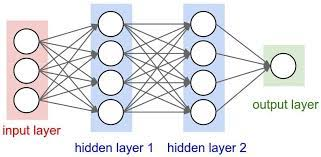
\includegraphics[width=0.95\textwidth]{ann.png}
	\end{minipage}	
\end{frame}
\note{
	Artificial Neural Networks or ANN is an information processing paradigm that is inspired by the way the biological nervous system such as brain process information. 
	It is composed of a large number of highly interconnected processing elements(neurons) working together in harmony to solve a specific problem such as regression, classification, image detection and identification and in time series data.
	A basic ANN is composed of three layers:\\
	the input layer, the hidden layer or layers and finally an output layer.
	Information flows from the input layer, through the hidden layer to the output layer.
}

\setcounter{subfigure}{0}
\begin{frame}{Convolutional neural networks}
	\begin{minipage}[c]{0.35\textwidth}
		\textbf{Convolution operation}\\
		\subfloat{\animategraphics[autoplay,loop, controls,width=4cm]{1}{figures/gif_figs/conv_op/conv_op-}{0}{8}}
	\end{minipage}
	\begin{minipage}[0]{0.6\textwidth}
		\subfloat{\includegraphics[[width=0.95\textwidth]{cnn.png}}
	\end{minipage}
	\tiny
	(source: https://github.com/tbozinis/simple-convolution)
\end{frame}
\setcounter{subfigure}{0}
%%%%%%%%%%%%%%%%%%%%%%%%%%%%%%%%%%%%%%%%%%%%%%%%%%
\begin{frame}{Training process}
	
	\begin{minipage}[ct]{0.4\textwidth}
			\begin{itemize}
				\footnotesize
				\item Feed-forward pass (initial predictions are done).
				\item Calculating the loss between the prediction and actual  values via optimization process e.g. (Gradient descent).
				\item Updating all learnable parameters using backpropagation technique.				
				\begin{equation}
					w_{jk}\leftarrow w_{jk}-\alpha \frac{\partial J}{\partial w_{jk}}					
				\end{equation}
				\begin{equation}										
					b_{jk}\leftarrow b_{jk}-\alpha \frac{\partial J}{\partial b_{jk}}
				\end{equation}
			\end{itemize}
		
	\end{minipage}
\hfill
	\begin{minipage}[c]{0.55\textwidth}
		\begin{figure}
			\centering
			\subfloat{\animategraphics[autoplay,loop, controls,width=6cm]{2}{figures/gif_figs/sgd/SGD.gif-}{0}{10}}
		\end{figure}
	\tiny
	(source: https://suniljangirblog.files.wordpress.com/2018/12/1-1.gif?w=379
	)
	\end{minipage}

\end{frame}
\begin{frame}{Why deep learning?}
	\centering
	\textbf{End-to-end approach} 
	\par\medskip
	\subfloat{\includegraphics[width=.95\textwidth]{DL_approach.png}}
\end{frame}
%%%%%%%%%%%%%%%%%%%%%%%%%%%%%%%%%%%%%%%%%%%%%%%%%%%%%%%%%%%%%%%%%%%%%%%%%%%%%%%%
\subsection{Computer vision}
\setcounter{subfigure}{0}
\begin{frame}{What is computer vision?}
	\begin{minipage}[c]{0.30\textwidth}
		Computer vision is a field of AI that enables computers and systems to derive meaningful information from digital images, videos and other visual inputs. 
	\end{minipage}
	\hfill
	\begin{minipage}[c]{0.65\textwidth}
		\begin{figure}
			\centering
			\includegraphics[width=1\textwidth]{computer_vision_tasks.png}
		\end{figure}
	\end{minipage}
\end{frame}
%%%%%%%%%%%%%%%%%%%%%%%%%%%%%%%%%%%%%%%%%%%%%%%%%%
\subsection{Synthetic Dataset generation}
\setcounter{subfigure}{0}
%%%%%%%%%%%%%%%%%%%%%%%%%%%%%%%%%%%%%%%%%%%%%%%%%%
\begin{frame}{Dataset description}
	\centering
	\begin{minipage}[c]{0.35\textwidth}
		\begin{itemize}
			\justifying
			\item 475 cases.
			\item Delamination has a different shape, size and location for each case.
			\item CFRP is made of 8-layers.
			\item Delamination was modelled between the 3rd and 4th layer.			
		\end{itemize}
	\end{minipage}
	\begin{minipage}[c]{0.6\textwidth}
		\begin{figure}
			\centering			
			\subfloat[Delamination orientation \label{fig:1}]{\includegraphics[width=0.52\textwidth]{figure1.png}}\qquad
			\subfloat[all cases overlapped \label{fig:2}]{\includegraphics[width=0.35\textwidth]{figure_overlap.png}}
		\end{figure}
	\end{minipage}
\end{frame}

\note{
	Dataset generation.
	Numerically generating 475 cases of full wavefield of propagating Lamb waves in a plate made of CFRP as shown in the figure. \\
	Essentially, the output resembles measurements acquired by SLDV in the transverse direction (perpendicular to the plate surface). \\
	Each delamination with different shape, size and location was modelled randomly on the plate.\\ 
	To improve the delamination visibility Root mean square RMS was applied.
	The dataset is used to train the deep learning models in order to identify the delaminations..
}
\setcounter{subfigure}{0}
\begin{frame}{Training Sample case}
	\begin{figure}
		\centering		
		\subfloat[Full wavefield \label{fig:3}]{\animategraphics[autoplay,loop, controls,width=4cm]{16}{figures/gif_figs/7_output/flat_shell_Vz_7_500x500bottom-}{1}{512}}\qquad
		\subfloat[RMS image \label{fig:4}]{\includegraphics[width=4cm]{RMS_flat_shell_Vz_7_500x500bottom.png}}\qquad
		\subfloat[Ground truth (label) \label{fig:5}]{\includegraphics[width=4cm]{m1_rand_single_delam_7.png}}
	\end{figure}
\end{frame}


\subsection{Semantic segmentation}
\setcounter{subfigure}{0}
\begin{frame}{Image semantic segmentation}
	\begin{minipage}[l]{0.35\textwidth}
		Segmentation schemes can be developed:
		\medskip
		\begin{enumerate}			
			\item \textbf{One-to-one \\(RMS based approach)} 
			\medskip
			\item \textbf{Many-to-one \\(Full wavefield frames)}
		\end{enumerate}
	\end{minipage}
	\begin{minipage}[l]{0.6\textwidth}
		\begin{figure}
			\centering
			\subfloat[Single input]{\includegraphics[width=.32\textwidth]{RMS_flat_shell_Vz_381_500x500bottom.png}}\qquad
			\subfloat[Single output]{\includegraphics[width=.32\textwidth]{GCN_381.png}}\qquad
			\\
			\subfloat[Full wavefield frames]{\animategraphics[autoplay,loop,width=.32\textwidth]{4}{figures/gif_figs/381_output/flat_shell_Vz_381_500x500bottom-}{85}{113}}\qquad
			\subfloat[Single output]{\includegraphics[width=.32\textwidth]{GCN_381.png}}
			
		\end{figure}
	\end{minipage}	
\end{frame}

\setcounter{subfigure}{0}
\subsection{Developed DL models}
\begin{frame}{Common deep learning architectures}
	
	\begin{minipage}[t]{0.45\textwidth}
		\textbf{RMS based}\\
		\begin{itemize}
			\item Convolutional neural networks (CNN)
			\item Fully convolutional network (FCN)
		\end{itemize}		
	\end{minipage}
	\hfill
	\begin{minipage}[t]{0.45\textwidth}
		\textbf{Full wavefield frames}\\
		\begin{itemize}
			\item Recurrent neural network (RNN)
			\item Long short-term memory (LSTM)
			\item ConvLSTM
		\end{itemize}	
	\end{minipage}
\end{frame}

%%%%%%%%%%%%%%%%%%%%%%%%%%%%%%%%%%%%%%%%%%%%%%%%%%
\begin{frame}{Developed model for delamination identification}
	\begin{minipage}[t]{0.45\textwidth}
		\textbf{RMS based models: \\}
			\begin{itemize}
				\item Res-UNet
				\item VGG 16 encoder-decoder
				\item FCN-DenseNet
				\item PSPNet
				\item GCN
			\end{itemize}
		{\tiny  
			\begin{enumerate}
				\item Ijjeh AA, Kudela P. Deep learning based segmentation using full wavefield processing for delamination identification: A comparative study. Mechanical Systems and Signal Processing. 2022 Apr 1;168:108671.
				\item Ijjeh AA, Ullah S, Kudela P. Full wavefield processing by using FCN for delamination detection. Mechanical Systems and Signal Processing. 2021 May 15;153:107537.
				
			\end{enumerate}}	
	\end{minipage}
	\hfill
	\begin{minipage}[t]{.45\textwidth}
	\textbf{Full wavefield frames based model:}
		\begin{itemize}
			\item Autoencoder ConvLSTM
		\end{itemize}
	\tiny
	\item Ullah S, Ijjeh AA, Kudela P. Deep learning approach for delamination identification using animation of Lamb waves. (submitted / under review)
	\end{minipage}
\end{frame}
%%%%%%%%%%%%%%%%%%%%%%%%%%%%%%%%%%%%%%%%%%%%%%%%%%
\setcounter{subfigure}{0}
\begin{frame}{RMS based models}
	\begin{minipage}[c]{0.55\textwidth}
		\begin{figure}
			\subfloat[Res-UNet model]{\includegraphics[width=1\textwidth]{figure4.png}}
		\end{figure}
	\end{minipage}
	\begin{minipage}[c]{0.35\textwidth}
		\begin{figure}
			\subfloat[Data flow \& intermediate outputs of layers \label{fig:}]{\animategraphics[autoplay, controls,width=.8\textwidth]{4}{figures/gif_figs/381__inter_pred/intermediate_output-}{0}{103}}
\end{figure}
	\end{minipage}

\end{frame}

%%%%%%%%%%%%%%%%%%%%%%%%%%%%%%%%%%%%%%%%%%%%%%%%%%
\setcounter{subfigure}{0}
\begin{frame}{Autoencoder ConvLSTM model}
	\begin{minipage}[c]{.4\textwidth}
	\begin{figure}
		\centering
		\includegraphics[width=.55\textwidth]{figure5b.png}
	\end{figure}
	\end{minipage}
	\begin{minipage}[c]{.55\textwidth}
	\begin{figure}
		\subfloat[Input frames]{\animategraphics[autoplay,loop,width=.40\textwidth]{4}{figures/gif_figs/381_output/flat_shell_Vz_381_500x500bottom-}{85}{113}}\qquad
		\subfloat[Prediction]{\includegraphics[width=.40\textwidth]{GCN_381.png}}\qquad
	\end{figure}
	\end{minipage}
	
\end{frame}
\setcounter{subfigure}{0}
\begin{frame}{Experimental results}
	\begin{minipage}[ct]{0.5\textwidth}
	\begin{figure}
		\centering
		\includegraphics[width=.95\textwidth]{figure3.png}
	\end{figure}
	\end{minipage}
	\hfill
	\begin{minipage}[t]{0.4\textwidth}
			\centering
			\subfloat{\animategraphics[autoplay,controls, loop,width=.40\textwidth]{12}{figures/gif_figs/exp/exp-}{0}{487}} 
			\par\medskip
			\subfloat{\includegraphics[width=.95\textwidth]{exp_rms_thresholded.png}}\qquad
	\end{minipage}
\end{frame}
%%%%%%%%%%%%%%%%%%%%%%%%%%%%%%%%%%%%%%%%%%%%%%%%%%
{\setbeamercolor{palette primary}{fg=blue, bg=white}
\begin{frame}[standout]
  Thank you for your listening!\\ \vspace{12pt}
  Questions?\\ \vspace{12pt}
  \url{aijjeh@imp.gda.pl}
\end{frame}
}
\note{Than you for listening, and I am  }
%%%%%%%%%%%%%%%%%%%%%%%%%%%%%%%%%%%%%%%%%%%%%%%%%%
% END OF SLIDES
%%%%%%%%%%%%%%%%%%%%%%%%%%%%%%%%%%%%%%%%%%%%%%%%%%
\end{document}